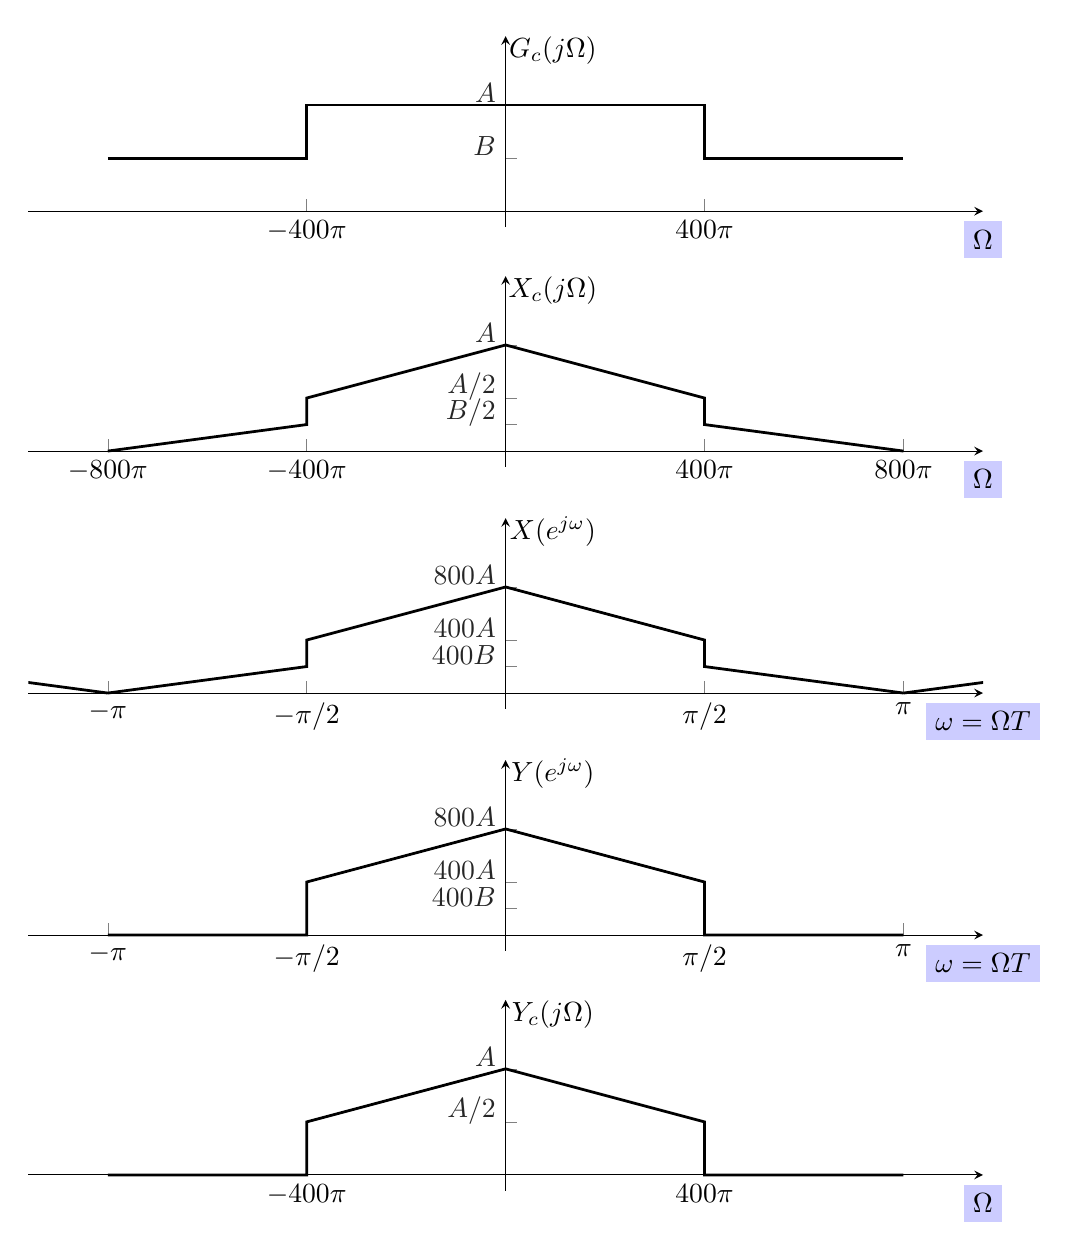
\begin{tikzpicture}
\begin{axis}[
	name=plot1,
	axis lines*=middle,
	enlargelimits = true,
	clip=true,
	scale only axis,
	width=\textwidth,
	height=0.2\textwidth,
	ymin=0, ymax=3,
	xmin=-8, xmax=8,
	axis line style={->,>=stealth},
	xlabel={\tikz[baseline]{\node[fill=blue!20,anchor=base] (t1) {$\Omega$};}},
	ylabel={$G_c(j\Omega)$},
	every axis x label/.style={
		at={(ticklabel* cs:1)},
		%xshift=0.2cm,
		anchor=north,
	},
	every axis y label/.style={
		at={(ticklabel* cs:0.8)},
		anchor=south,
		xshift=0.6cm,
	},
	ytick={1, 2},
	yticklabels={$B$, $A$},
	yticklabel style={yshift=0.15cm},
	xtick={-4, 4},
	xticklabels={$-400\pi$, $400\pi$}, 
	every outer y axis line/.append style={white!15!black},
	every y tick label/.append style={font=\color{white!15!black}},
	legend style={draw=white!15!black,fill=white,legend cell align=left}]
	\addplot[solid, line width=1pt] coordinates {(-8, 1) (-4, 1) (-4, 2) (4, 2) (4, 1) (8, 1)};
\end{axis}

\begin{axis}[
name=plot2,
at=(plot1.below south east), anchor=above north east,
axis lines*=middle,
enlargelimits = true,
clip=true,
scale only axis,
width=\textwidth,
height=0.2\textwidth,
ymin=0, ymax=3,
xmin=-8, xmax=8,
axis line style={->,>=stealth},
xlabel={\tikz[baseline]{\node[fill=blue!20,anchor=base] (t1) {$\Omega$};}},
ylabel={$X_c(j\Omega)$},
every axis x label/.style={
	at={(ticklabel* cs:1)},
	%xshift=0.2cm,
	anchor=north,
},
every axis y label/.style={
	at={(ticklabel* cs:0.8)},
	anchor=south,
	xshift=0.6cm,
},
ytick={0.5, 1, 2},
yticklabels={$B/2$, $A/2$, $A$},
yticklabel style={yshift=0.15cm},
xtick={-8, -4, 4, 8},
xticklabels={$-800\pi$, $-400\pi$, $400\pi$, $800\pi$}, 
every outer y axis line/.append style={white!15!black},
every y tick label/.append style={font=\color{white!15!black}},
legend style={draw=white!15!black,fill=white,legend cell align=left}]
\addplot[solid, line width=1pt] coordinates {(-8, 0) (-4, 1/2) (-4, 1) (0, 2) (4, 1) (4, 1/2) (8, 0)};
\end{axis}

\begin{axis}[
name=plot3,
at=(plot2.below south east), anchor=above north east,
axis lines*=middle,
enlargelimits = true,
clip=true,
scale only axis,
width=\textwidth,
height=0.2\textwidth,
ymin=0, ymax=3,
xmin=-8, xmax=8,
axis line style={->,>=stealth},
xlabel={\tikz[baseline]{\node[fill=blue!20,anchor=base] (t1) {$\omega = \Omega T$};}},
ylabel={$X(e^{j\omega})$},
every axis x label/.style={
	at={(ticklabel* cs:1)},
	%xshift=0.2cm,
	anchor=north,
},
every axis y label/.style={
	at={(ticklabel* cs:0.8)},
	anchor=south,
	xshift=0.6cm,
},
ytick={0.5, 1, 2},
yticklabels={$400B$, $400A$, $800A$},
yticklabel style={yshift=0.15cm},
xtick={-8, -4, 4, 8},
xticklabels={$-\pi$, $-\pi/2$, $\pi/2$, $\pi$}, 
every outer y axis line/.append style={white!15!black},
every y tick label/.append style={font=\color{white!15!black}},
legend style={draw=white!15!black,fill=white,legend cell align=left}]
\addplot[solid, line width=1pt] coordinates {(-8, 0) (-4, 1/2) (-4, 1) (0, 2) (4, 1) (4, 1/2) (8, 0)};
\addplot[solid, line width=1pt] coordinates {(-8+16, 0) (-4+16, 1/2) (-4+16, 1) (0+16, 2) (4+16, 1) (4+16, 1/2) (8+16, 0)};
\addplot[solid, line width=1pt] coordinates {(-8-16, 0) (-4-16, 1/2) (-4-16, 1) (0-16, 2) (4-16, 1) (4-16, 1/2) (8-16, 0)};
\end{axis}

\begin{axis}[
name=plot4,
at=(plot3.below south east), anchor=above north east,
axis lines*=middle,
enlargelimits = true,
clip=true,
scale only axis,
width=\textwidth,
height=0.2\textwidth,
ymin=0, ymax=3,
xmin=-8, xmax=8,
axis line style={->,>=stealth},
xlabel={\tikz[baseline]{\node[fill=blue!20,anchor=base] (t1) {$\omega = \Omega T$};}},
ylabel={$Y(e^{j\omega})$},
every axis x label/.style={
	at={(ticklabel* cs:1)},
	%xshift=0.2cm,
	anchor=north,
},
every axis y label/.style={
	at={(ticklabel* cs:0.8)},
	anchor=south,
	xshift=0.6cm,
},
ytick={0.5, 1, 2},
yticklabels={$400B$, $400A$, $800A$},
yticklabel style={yshift=0.15cm},
xtick={-8, -4, 4, 8},
xticklabels={$-\pi$, $-\pi/2$, $\pi/2$, $\pi$}, 
every outer y axis line/.append style={white!15!black},
every y tick label/.append style={font=\color{white!15!black}},
legend style={draw=white!15!black,fill=white,legend cell align=left}]
\addplot[solid, line width=1pt] coordinates {(-8, 0) (-4, 0) (-4, 1) (0, 2) (4, 1) (4, 0) (8, 0)};
\end{axis}

\begin{axis}[
name=plot5,
at=(plot4.below south east), anchor=above north east,
axis lines*=middle,
enlargelimits = true,
clip=true,
scale only axis,
width=\textwidth,
height=0.2\textwidth,
ymin=0, ymax=3,
xmin=-8, xmax=8,
axis line style={->,>=stealth},
xlabel={\tikz[baseline]{\node[fill=blue!20,anchor=base] (t1) {$\Omega$};}},
ylabel={$Y_c(j\Omega)$},
every axis x label/.style={
	at={(ticklabel* cs:1)},
	%xshift=0.2cm,
	anchor=north,
},
every axis y label/.style={
	at={(ticklabel* cs:0.8)},
	anchor=south,
	xshift=0.6cm,
},
ytick={1, 2},
yticklabels={$A/2$, $A$},
yticklabel style={yshift=0.15cm},
xtick={-4, 4},
xticklabels={$-400\pi$, $400\pi$}, 
every outer y axis line/.append style={white!15!black},
every y tick label/.append style={font=\color{white!15!black}},
legend style={draw=white!15!black,fill=white,legend cell align=left}]
\addplot[solid, line width=1pt] coordinates {(-8, 0) (-4, 0) (-4, 1) (0, 2) (4, 1) (4, 0) (8, 0)};
\end{axis}

\end{tikzpicture}
